\section{Our Approach}
\label{sec:approach}
Our main idea is to decompose \textbf{TIP} into $|H|$ subproblems,
each resolving a single contact in $H$.
To solve a contact of $i$ and $j$ at time $t$, we consider the locations
of their last contacts. The key observation is that even though
there can be many possible traces spanning from the previous locations
of $i$ and $j$, only a small number of them can produce the contact,
due to the distance constraints of the map.

Fig.\ref{fig:des} illustrates this approach.
Suppose nodes $A$, $B$ and $C$ starts their movements at $t_0$ from point $A$, $B$ and $C$
in the diagram. $A$ and $B$ contact at $t_1$. Given $A$'s speed, we know by $t_1$, there are
5 possible traces for $A$ ending at $A1$-$A5$ respectively. Similarly, $B$ has 6 possible traces
and 5 locations up to time $t_1$. Of all 15 pairs of traces between $A$ and $B$, only 4
pairs of traces satisfy the contact constraint, which may occur at locations marked by ($A1$, $B1$),
($A4$, $B3$) and ($A2$/$A3$, $B2$). The rest of the traces are pruned and not considered further.
In the next round, $B$ and $C$ contact at time $t_2$. We repeat the above process,
using $B1$, $B2$ and $B3$ as the $B$'s initial locations for this round. As the figure shows,
the only possible trace for $B$ left is $B1 \rightarrow B6$ given the short time interval between $t_1$ and
$t_2$.

\begin{figure}[th]
\centering
\epsfig{file=contact-example.eps, width=0.7\columnwidth}
\caption{Inference of a Short Contact History}
\label{fig:des}
\end{figure}


Since the time interval $t$ between two successive contacts of $i$ and $j$ follows the exponential distribution
\[P\{t\leq x\}=1-e^{-\lambda_{ij} x}, x\in[0,\infty)\]
where $\lambda_{ij}$ is the contact rate between $i$ and $j$, the expected contact interval between $i$ and $j$
is $E[t]=\frac{1}{\lambda_{ij}}$. Let $\lambda_{ij}$ be its mean value $\bar{\lambda}$,
the number of contacts $|H|$ is
\begin{equation*}
|H| =  \frac{1}{2}\sum_i\sum_{j\not=i} t_{max}/\frac{1}{\lambda_{ij}}
\approx\frac{1}{2}\bar{\lambda} t_{max}|N|^2
\label{equ:complexity}
\end{equation*}
Let $t_{c}$ be the expected time to infer each contact.
If the contact interval of all nodes is bounded then $t_{c}$
is also bounded. Therefore, the time cost of our
approach is linear to $|H|$, which is also linear to
$t_{max}$ and $|N|^2$.

\subsection{exactly meet on a fixed point}
Though bluetooth communication range is about 10m, it is still omitted due to its marginal ratio to the scale of the map.
On the other hand, we will show that it is reasonable to assume meeting exactly on a fixed point.

As we defined, the trace $l_i(t)$ of a node is the location sequence of the time. Given a location point $l=(x,y)$ on the map, we assume that $i$ is at $l$($l_i(t)=l$) when $i$ meets $j$, then $l_j(t)$ is
\[l_j(t)  =  \arg\max_{l_j} P\{l_j(t)|l_i(t)=l\}\]
\[ = \arg\max_{l_j} \frac{P\{l_i(t) = l|l_j(t)\}\cdot P\{l_j(t)\}}{P\{l_i(t)=l\}}\]
where $P\{l_i(t)=l\}$ is determined as we assume $l_i(t)=l$, 

 
\subsection{entropy bound}